\newcommand{\chapter}[2][]{
	\newcommand{\chapname}{#2}
	\begin{flushleft}
		\begin{minipage}[t]{\linewidth}
			
\includegraphics[height=1cm]{hdht-logo.png}
			\hspace{0pt}	
			\sffamily\bfseries\large Bài 2.
			\begin{flushleft}
				\Large\bfseries #1
			\end{flushleft}
		\end{minipage}
	\end{flushleft}
	\vspace{1cm}
	\normalfont\normalsize
}
\chapter[Giới thiệu các lĩnh vực nghiên cứu trong Vật lí học:\\ - Thiên văn và năng lượng cao \\-  Nano và Laser \\- Bán dẫn và Y sinh]{Giới thiệu các lĩnh vực nghiên cứu trong Vật lí học:\\ Thiên văn và năng lượng cao - Nano và Laser \\- Bán dẫn và Y sinh}
\section{Hình thành kiến thức mới}

\subsection{Hình thành kiến thức mới}
\subsubsection{Lĩnh vực thiên văn và vũ trụ học}
Thiên văn học nghiên cứu về các tiến trình phát triển trong vũ trụ và nhận dạng các mối quan hệ trong những tiến trình đó.

Thời cổ đại, con người đã quan sát bầu trời để phục vụ các hoạt động nông nghiệp và đời sống. Tuy nhiên, hầu hết các ứng dụng đều dựa trên kinh nghiệm và thực tiễn quan sát mà chưa hệ thống hóa thành lí luận, hoặc có lí luận nhưng cũng chỉ dựa vào kinh nghiệm và thực tiễn quan sát.

Từ thế kỉ XVI, sự ra đời của kính viễn vọng (kính thiên văn) cùng với phương pháp phân tích quang phổ đã đặt nền móng cho quang phổ học (một phương pháp quan trọng để nghiên cứu về tính chất, nhiệt độ, tuổi thọ, thành phần cấu tạo của các thiên thể).

Ngày nay, mục đích của thiên văn học là tìm hiểu quá trình hình thành và phát triển của vũ trụ. Lí thuyết Big Bang đang được công nhận là thuyết phù hợp nhất để giải thích về sự hình thành và phát triển của vũ trụ. Theo lí thuyết này thì vũ trụ khởi thủy từ một điểm đặc, nóng (mật độ vật chất vô hạn, nhiệt độ vô hạn). Vì một lí do nào đó, vụ nổ lớn xảy ra và từ đó vũ trụ không ngừng dãn nở, kèm theo đó là sự giảm nhiệt độ trên toàn vũ trụ.
\begin{center}
	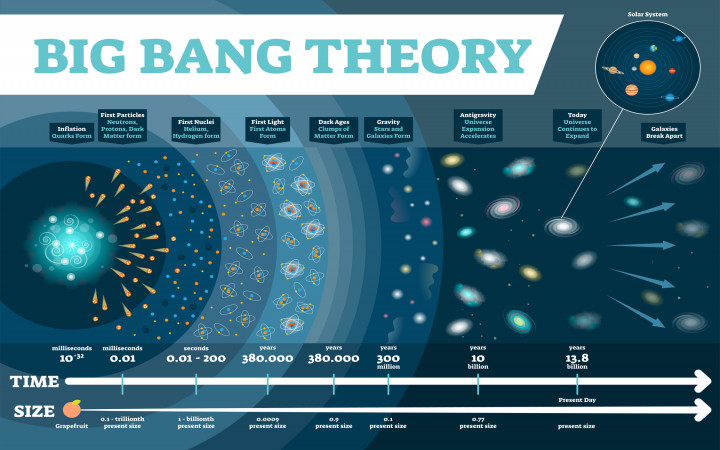
\includegraphics[scale=0.7]{../figs/G10-002-1.jpg}
\end{center}
Về các phương tiện quan sát vũ trụ, con người không chỉ chế tạo các thiết bị quan sát bầu trời từ mặt đất, mà còn có các con tàu vũ trụ và trạm vũ trụ để quan sát từ bên ngoài Trái Đất (kính viễn vọng Hubble, tàu vũ trụ Vostok).

\begin{minipage}[l]{0.6\textwidth}
Các hướng nghiên cứu chủ yếu của lĩnh vực thiên văn và vũ trụ học:
\begin{itemize}
	\item Thiên văn: Nghiên cứu các thiên thể và các hiện tượng tự nhiên có nguồn gốc ngoài Trái Đất;
	\item Công nghệ vệ tinh: Nghiên cứu, thiết kế, chế tạo, vận hành vệ tinh đưa vào không gian để phục vụ truyền thông, liên lạc, ...
	\item Viễn thám: Đo đạc, thu thập, nghiên cứu, xử lí thông tin và các đối tượng trên bề mặt Trái Đất và khí quyển thông qua các ảnh chụp từ vệ tinh trên phạm vi rộng lớn.
\end{itemize}
\end{minipage}
\begin{minipage}[r]{0.4\textwidth}
\begin{center}
	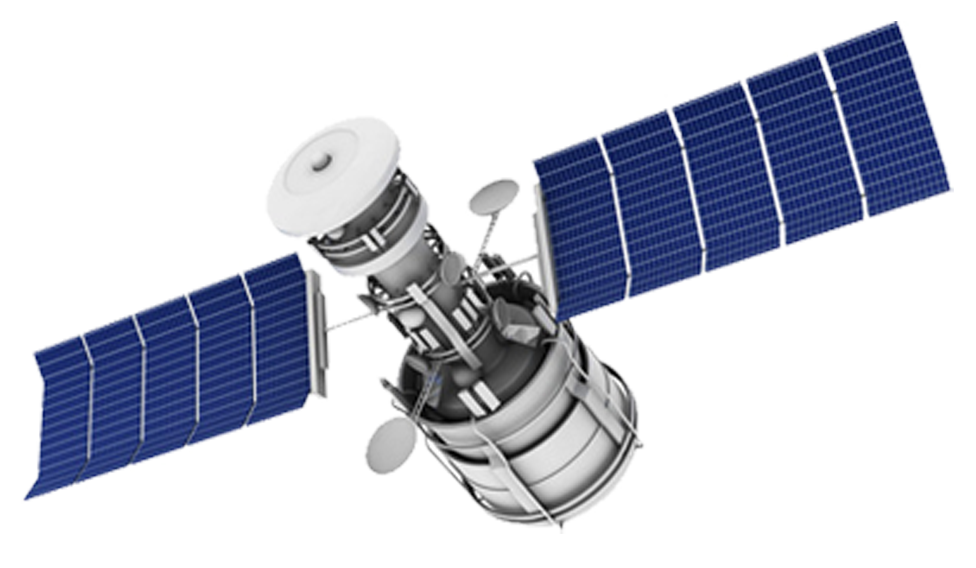
\includegraphics[scale=0.1]{../figs/G10-002-2.png}
\end{center}
\begin{center}
	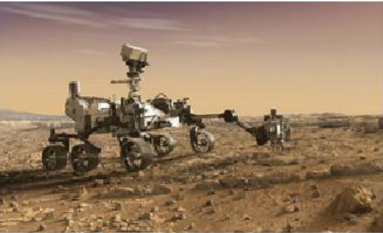
\includegraphics[scale=0.7]{../figs/G10-002-3.png}
\end{center}
\end{minipage}

\subsubsection{Lĩnh vực Vật lí hạt cơ bản (Vật lí năng lượng cao)}
Vật lí hạt cơ bản nghiên cứu về các hạt cơ bản (các hạt sơ cấp) chứa trong vật chất và những tương tác giữa chúng.

\begin{minipage}[l]{0.6\textwidth}
Ý tưởng về vật chất được cấu tạo từ các hạt nhỏ bé, không phân chia được, đã được đưa ra từ thế kỉ VI trước Công nguyên. Cho đến năm 1810, Dalton mới đưa ra được luận điểm chứng minh sự tồn tại của nguyên tử. Theo thuyết của Dalton, nguyên tử là hạt nhỏ nhất và không thể phân chia được nữa.
\end{minipage}
\begin{minipage}[r]{0.4\textwidth}
\begin{center}
	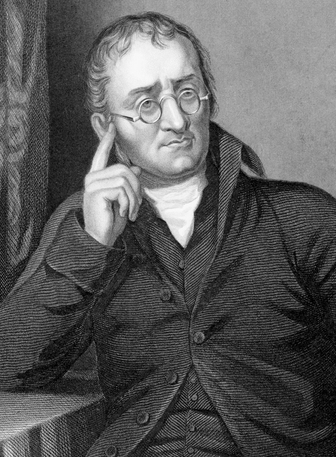
\includegraphics[scale=0.4]{../figs/G10-002-5.png}
\end{center}
\end{minipage}

Vào những năm 1930, các nhà khoa học đã khám phá và chứng minh được rằng: có hai loại hạt, hạt cơ bản là những hạt không thể phân chia nhỏ hơn được nữa và hạt tổ hợp là những hạt được cấu thành bởi các hạt khác.

Các nghiên cứu trong Vật lí hiện đại tập trung vào những hạt có cấu trúc nhỏ hơn nguyên tử.

Nhiều hạt cơ bản không xuất hiện trong môi trường tự nhiên, chúng chỉ tồn tại trong những điều kiện đặc biệt được tạo ra từ phòng thí nghiệm với thời gian tồn tại rất ngắn. Để xuất hiện những hạt này, các nhà khoa học sử dụng những máy gia tốc hạt, nhằm cung cấp động năng tương đối lớn để các phản ứng xảy ra. Do đó, Vật lí hạt cơ bản còn được gọi là Vật lí năng lượng cao.

Bên cạnh các thiết bị đặc biệt dùng trong thí nghiệm, các nhà khoa học còn đề ra những mô hình lí thuyết để giải thích và tiên đoán sự xuất hiện của các hạt thí nghiệm, đặc biệt phải kể đến mô hình chuẩn.

\begin{center}
	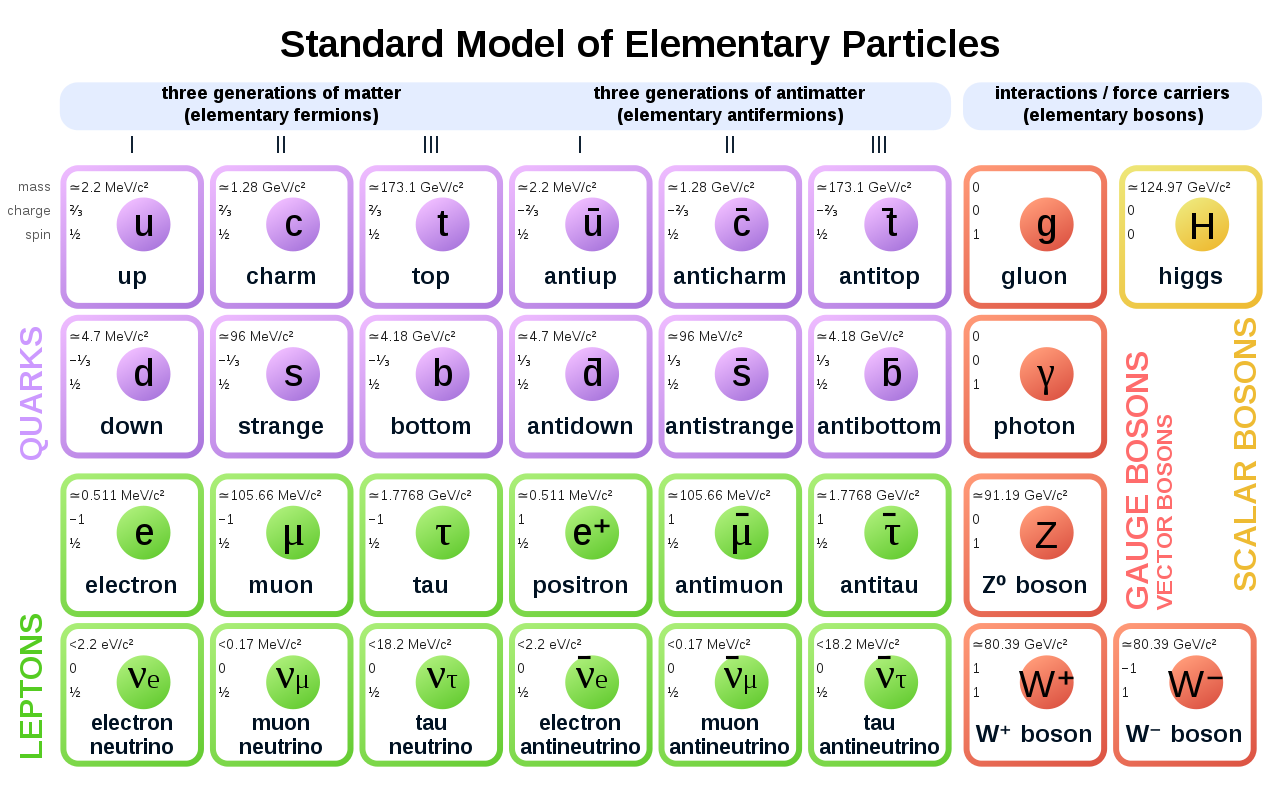
\includegraphics[scale=0.3]{../figs/G10-002-4.png}
\end{center}

Mô hình chuẩn phân loại các hạt cơ bản theo 4 loại tương tác tự nhiên và số lượng tử của chúng, đồng thời còn đưa ra dự đoán về sự tồn tại của các hạt chưa được phát hiện. Có thể nói, mô hình chuẩn có chức năng như Bảng hệ thống tuần hoàn dùng trong Vật lí hạt cơ bản.
\subsubsection{Lĩnh vực Vật lí nano}
Vật lí nano là lĩnh vực nghiên cứu liên ngành trong Vật lí, được hình thành trong những năm đầu của thế kỉ XX. Vật lí nano nghiên cứu vật chất hay các thiết bị có kích thước từ 1 đến 100 nm. Ở kích thước này, các nguyên tắc vật lí và hóa học cổ điển không thể được áp dụng để giải thích các hiện tượng quan sát được một cách chính xác.

\begin{minipage}[l]{0.6\textwidth}
Vật lí nano có thể được chia thành hai ngành nhỏ hơn là khoa học nano và công nghệ nano.
\begin{itemize}
	\item Khoa học nano nghiên cứu các tính chất vật lí, hóa học đặc biệt của các loại vật liệu ở cấp độ nanômét.
	\item Công nghệ nano tập trung triển khai những thành tựu nghiên cứu của khoa học nano vào các ứng dụng thực tế.
\end{itemize}
\end{minipage}
\begin{minipage}[r]{0.4\textwidth}
\begin{center}
	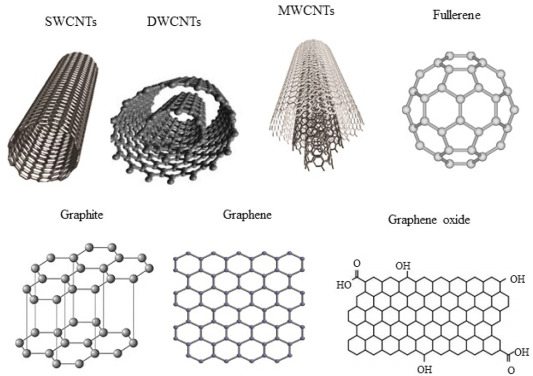
\includegraphics[scale=0.4]{../figs/G10-002-6}
\end{center}
\end{minipage}

Thành tựu của Vật lí nano thúc đẩy phát triển công nghệ nano liên quan đến việc thiết kế, phân tích, chế tạo và sử dụng vật liệu ở kích cỡ nano, làm tăng và tạo ra tính chất đặc biệt của vật liệu, ... ứng dụng trong mọi lĩnh vực từ đời sống đến sản xuất và môi trường.
\subsubsection{Lĩnh vực Vật lí LASER}
LASER là từ viết tắt tiếng Anh của ``Light Amplification by Stimulated Emmision of Radiation'' (sự khuếch đại ánh sáng bằng bức xạ cảm ứng), là nguồn sáng thu được nhờ sự khuếch đại ánh sáng bằng bức xạ phát ra khi kích hoạt các phần tử của môi trường vật chất.

LASER là ánh sáng có nhiều tính chất đặc biệt: tập trung năng lượng rất lớn, có tính đơn sắc và định hướng cao.

Năm 1960, nhà Vật lí Theodore H. Maiman đã thành công trong việc chế tạo bộ phát LASER đầu tiên trên thế giới khi sử dụng hông ngọc làm môi trường hoạt tính.



Ngày nay, tia LASER có thể được tạo ra từ nhiều môi trường hoạt tính khác nhau tùy theo mục đích sử dụng:
\begin{itemize}
	\item LASER khí: He-Ne, CO$_2$, $\ldots$;
	\item LASER rắn: Ti-Sapphire, Rubidium;
	\item LASER chất bán dẫn.
\end{itemize}

\begin{minipage}[l]{0.6\textwidth}
Đối tượng nghiên cứu trong Vật lí LASER rất phong phú và đa dạng:
\begin{itemize}
	\item Nghiên cứu cấu trúc của nguyên tử, phân tử thông qua các hiệu ứng quang phi tuyến;
	\item Nghiên cứu để quan sát sự hình thành các liên kết hóa học trong thời gian rất ngắn bằng cách sử dụng những xung LASER cực ngắn nhằm tạo ra độ phân giải phù hợp;
	\item Nghiên cứu chế tạo các thiết bị quang học, quang - điện tử mới có những tính năng vượt trội;
	\item Nghiên cứu chế tạo công cụ, thiết bị để bẫy nguyên tử hay các hạt có kích thước từ micrômét đến nanômét;
	\item Nghiên cứu phát triển công nghệ chụp ảnh cấu trúc vật liệu mà không phá hủy mẫu vật;
	\item Nghiên cứu phát triển các công nghệ mới để chẩn đoán và điều trị trong lĩnh vực y học.
\end{itemize}
\end{minipage}
\begin{minipage}[r]{0.4\textwidth}
\begin{center}
	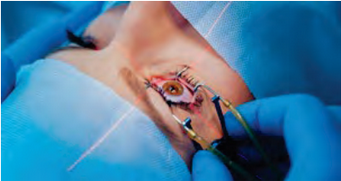
\includegraphics[scale=0.6]{../figs/G10-002-7}
\end{center}
\begin{center}
	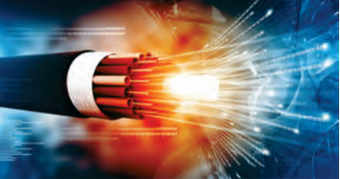
\includegraphics[scale=0.6]{../figs/G10-002-8}
\end{center}
\begin{center}
	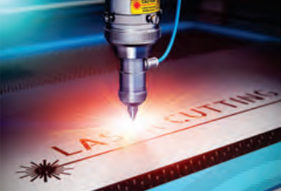
\includegraphics[scale=0.7]{../figs/G10-002-9}
\end{center}
\end{minipage}
\subsubsection{Lĩnh vực Vật lí bán dẫn}
Vật lí bán dẫn là lĩnh vực nghiên cứu những tính chất và cơ chế Vật lí xảy ra trong các chất bán dẫn.

\begin{minipage}[l]{0.6\textwidth}
Vật liệu bán dẫn trở thành vật liệu chủ yếu trong kĩ thuật điện tử hiện đại. Do vật liệu bán dẫn có thể chế tạo được các linh kiện rất nhỏ, vì vậy người ta đã dùng vật liệu này để chế tạo ra các mạch tổ hợp (mạch IC) hoặc các mạch IC siêu lớn. Trên các mạch IC siêu lớn có hàng chục nghìn linh kiện bán dẫn nhỏ, giúp cho thiết kế các máy tính, điện thoại nhỏ gọn hơn.
\end{minipage}
\begin{minipage}[r]{0.4\textwidth}
\begin{center}
	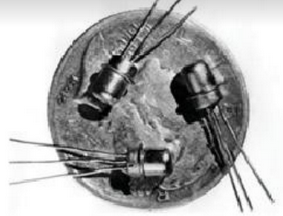
\includegraphics[scale=0.4]{../figs/G10-002-11}
\end{center}
\begin{center}
	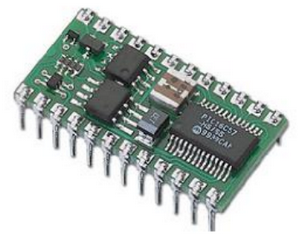
\includegraphics[scale=0.4]{../figs/G10-002-12}
\end{center}
\end{minipage}

Nhờ đặc tính nhạy sáng và nhiệt độ của vật liệu bán dẫn, người ta có thể chế tạo các cảm biến dùng trong các hệ thống điều khiển tự động.
\subsubsection{Lĩnh vực Vật lí y sinh}
Vật lí y sinh là môn khoa học liên ngành, ứng dụng lí thuyết và phương pháp của khoa học vật lí vào sinh học, y học. Nghiên cứu các hiện tượng xảy ra trong các tổ chức và cơ thể sống dựa trên những thành tựu của Vật lí.

Nội dung nghiên cứu của Vật lí y sinh rất rộng, như cơ chế sinh bệnh và tác dụng của các yếu tố từ môi trường và các yếu tố vật lí, các kĩ thuật chẩn đoán và điều trị bệnh hiện đại. Những năm gần đây, Vật lí y sinh còn nghiên cứu chế tạo thiết bị hỗ trợ, phục hồi chức năng vận động và thiết bị nano để điều hòa chức năng sinh học.

Cùng với sự phát triển của máy vi tính, Vật lí y sinh cũng nghiên cứu các kĩ thuật thí nghiệm và chẩn đoán bằng hình ảnh, có thể quan sát gián tiếp hoặc mô hình hóa cấu trúc và tương tác của từng phân tử hay nhiều phân tử.
\subsection{Mở rộng}
\subsubsection{Một số sản phẩm công nghệ ứng dụng Vật lí hiện đại đã từng được các thế hệ học sinh Việt Nam sáng chế}
Hà Nội: Học sinh lớp 8 chế tạo cánh tay robot điều khiển bằng suy nghĩ;

Cần Thơ: Học sinh lớp 10 chế tạo máy phát sóng siêu âm;

Quảng Nam: Học sinh lớp 11 chế tạo máy đo thân nhiệt tự động;

Nghệ An: Học sinh lớp 11 chế tạo xe lăn vượt địa hình;

KonTum: Học sinh lớp 12 chế tạo máy giám sát người đeo khẩu trang nơi công cộng;

Hà Nội: Nhóm sinh viên ứng dụng AI để hỗ trợ và kết nối người già;

Đồng Nai: Nhóm sinh viên nghiên cứu cửa chống trộm;

TPHCM: Nhóm sinh viên nghiên cứu "biến" bùn giấy thành vật liệu siêu bền.

Ngoài ra, vẫn còn rất nhiều ứng dụng hữu ích do học sinh, sinh viên chế tạo đã giành được nhiều giải thưởng lớn trong các Cuộc thi Khoa học kỹ thuật các cấp.

\subsubsection{Một số ngành đào tạo đại học ứng dụng các thành tựu của Vật lí hiện đại ở Việt Nam hiện nay}
Kĩ sư ngành Kĩ thuật hạt nhân: nghiên cứu cơ bản và ứng dụng liên quan đến bức xạ hạt nhân, thực hiện các công việc liên quan đến thiết kế, chế tạo, vận hành, bảo trì bảo dưỡng các thiết bị, hệ thống ứng dụng bức xạ hạt nhân trong y tế, công nghiệp, nông nghiệp.

Kĩ sư ngành Công nghệ kĩ thuật nano có khả năng làm việc trong nhiều lĩnh vực, họ có thể làm việc ở các cơ sở y tế, cơ sở sản xuất, kiểm tra chất lượng sản phẩm, nghiên cứu và phát triển sản phẩm, $\ldots$

Kĩ sư chuyên ngành Vật lí laser có cơ hội làm việc tại các trường đại học, viện nghiên cứu hoặc đơn vị nghiên cứu có liên quan trong ngành quang học, trong các cơ sở y tế viễn thông, các cơ sở thiết kế, chế tạo thiết bị và linh kiện quang học.

Các ngành đào tạo về Vật lí y sinh chuẩn bị cho sinh viên một nghề nghiệp như một nhà Vật lí trong y học và sinh học. Kĩ sư Vật lí y sinh có thể đảm nhận tốt công việc chuyên môn tại các bệnh viện, viện nghiên cứu, trường đại học, các công ty về thiết bị y tế, các trung tâm kiểm tra chất lượng thiết bị y tế, cơ quan quản lí nhà nước về an toàn bức xạ, $\ldots$
\section{Mục tiêu bài học - Ví dụ minh họa}
\begin{dang}{Nêu được đối tượng nghiên cứu của một số lĩnh vực chính của Vật lí hiện đại}
	\viduii{3}{Dựa vào sách báo và Internet, em hãy cho biết những giải thưởng Nobel về Vật lí trong những năm gần đây thuộc lĩnh vực gì? Từ đó kết luận về tính đa dạng trong nghiên cứu Vật lí của các nhà khoa học hiện nay.
	}
	{	\begin{center}
			\textbf{Hướng dẫn trả lời}
		\end{center}
		
		Nobel Vật lí năm 2021: nghiên cứu trong lĩnh vực khí hậu, các hệ vật lí từ nguyên tử đến hành tinh;
		
		Nobel Vật lí năm 2020: nghiên cứu về lỗ đen và thuyết tương đối tổng quát, vật thể nén đặc siêu khối lượng tại tâm Dải ngân hà;
		
		Nobel Vật lí năm 2019: nghiên cứu về vũ trụ;
		
		Nobel Vật lí năm 2018: những sáng chế đột phá trong lĩnh vực Vật lí laser;
		
		Nobel Vật lí năm 2017: LIGO và sóng hấp dẫn;
		
		Nobel Vật lí năm 2016, 2015: nghiên cứu trong lĩnh vực hạt cơ bản và năng lượng cao;
		
		Năm 2014: phát minh bóng LED lam;
		
		...
		
	}
	\viduii{3}{Dựa vào những hiểu biết của em, hãy so sánh sự khác nhau về đối tượng nghiên cứu giữa Vật lí cổ điển và Vật lí hiện đại.
	}
	{	\begin{center}
			\textbf{Hướng dẫn trả lời}
		\end{center}
		
	Vật lí cổ điển nghiên cứu các hiện tượng trong đời sống hàng ngày: vật chuyển động với vận tốc rất nhỏ so với vận tốc ánh sáng, trong những khoảng cách và kích thước lớn hơn nhiều thang đo nguyên tử.
	
	Thuật ngữ Vật lí hiện đại chỉ những khái niệm vật lí có liên quan đến tính lượng tử hóa của vật chất và sự biến đổi không thời gian và năng lượng dựa trên khái niệm về trường và vật lí thống kê.
		
	}
\end{dang}
\begin{dang}{Liệt kê được một vài mô hình lí thuyết đơn giản, một số phương pháp thực nghiệm của một số lĩnh vực chính của Vật lí hiện đại}
	\viduii{3}{Dựa vào sách báo và Internet, em hãy trình bày một số mô hình nguyên tử đã từng được các nhà khoa học đề xuất và công nhận.
	}
	{	\begin{center}
			\textbf{Hướng dẫn giải}
		\end{center}
		
		Một số mô hình phổ biến và đã được các nhà khoa học công nhận rộng rãi về cấu tạo nguyên tử có thể kể đến:
		\begin{itemize}
			\item Mô hình nguyên tử của Dalton;
			\item Mô hình nguyên tử của Thomson;
			\item Mô hình nguyên tử của Rutherford;
			\item Mô hình nguyên tử hidro của Borh;
			\item Mô hình Orbital nguyên tử.
		\end{itemize}
		
	}
	\viduii{3}{Dựa vào sách báo và Internet, em hãy tìm hiểu về sự tiến hóa của vũ trụ và quá trình phát hiện các hạt sơ cấp.
	}
	{	\begin{center}
			\textbf{Hướng dẫn trả lời}
		\end{center}
		
		Về sự tiến hóa vũ trụ, các em cần trả lời được về nguồn gốc vũ trụ, cấu tạo và đặc trưng của vũ trụ ở các mốc thời gian kể từ khi vũ trụ hình thành, các giả thuyết về nguyên nhân gây ra Vụ nổ lớn và thuyết Đa vũ trụ, ...
		
		Về quá trình phát hiện các hạt sơ cấp, các em cần nắm được thời điểm và phương pháp mà các nhà khoa học phát hiện các loại hạt, cách phân loại và thống kê các hạt sơ cấp theo các nhóm đặc trưng, khái niệm về các số lượng tử và sự tương tác của các hạt, ...
	}
\end{dang}